\documentclass[11pt]{article}
\usepackage{xcolor}
\usepackage{amsmath, amssymb, graphicx, cite}
\usepackage{hyperref}
\usepackage[margin=1in]{geometry}
\usepackage{setspace}
\usepackage{subfigure}
\usepackage{subcaption}
\usepackage{graphicx}
\doublespacing

% Custom colors
\definecolor{instr}{RGB}{0,0,180}
\definecolor{todo}{RGB}{0,100,0}
\newcommand{\instr}[1]{\textcolor{instr}{#1}}
\newcommand{\todo}[1]{\textcolor{todo}{#1}}

\title{\textbf{ERpy: Python Implementation of Entropic Regression for Nonlinear System Identification}}
\author{
Emanuele Bossi$^{1}$\\[6pt]
\small $^{1}$Department of Mathematics, Embry-Riddle Aeronautical University, Prescott, AZ
}
\date{\today}

\begin{document}

\maketitle

\begin{abstract}
Entropic Regression (ER) is an information-theoretic framework for sparse model discovery that leverages mutual information and conditional mutual information to identify relevant functional dependencies in dynamical systems \cite{almomani2020entropic}. In ER, these information-theoretic quantities are evaluated in conjunction with regression fitting, where dependencies are assessed through residual-based relationships rather than direct variable comparisons. Despite its potential, accessible and lightweight implementations of ER in Python are currently limited, hindering reproducibility and integration with modern data-driven workflows.

In this paper, we present \texttt{ERpy}, a concise and faithful Python implementation of the Entropic Regression framework that replicates the original methodology. This implementation aims to facilitate reproducibility, support rapid experimentation, and enable broader adoption of Entropic Regression within the scientific and engineering communities.

The entire codebase is released under the MIT license and is available on GitHub at \url{https://github.com/bossiemanuele/ERpy}.

\end{abstract}

\section{Introduction} \label{section1}
The discovery of governing equations from data has emerged as a central problem in the study of dynamical systems, with applications spanning physics, engineering, and complex networked systems \cite{brunton2022modern}. In recent years, data-driven approaches have gained significant attention as alternatives to purely first-principles modeling, particularly in scenarios where the underlying dynamics are partially unknown or difficult to derive analytically. A key challenge in this context is the identification of sparse and interpretable models that accurately capture the essential structure of the system while avoiding overfitting.

A prominent line of work in this area focuses on sparse regression techniques for system identification, where candidate libraries of nonlinear functions are constructed and sparse optimization is used to select the most relevant terms. One of the most influential approaches is \emph{Sparse Identification of Nonlinear Dynamics (SINDy)}, which demonstrated that parsimonious governing equations can be recovered from data using sparse regression methods \cite{brunton2016discovering}. Variants and extensions of this framework have since been applied across a wide range of scientific domains \cite{kaiser2018sindy}.

Among alternative approaches, \emph{Entropic Regression (ER)} introduces an information-theoretic perspective to model discovery \cite{almomani2020entropic}. Instead of relying solely on regression-based sparsity promotion, ER leverages mutual information (MI) and conditional mutual information (CMI) to quantify statistical dependencies between candidate functions and the target dynamics. Information-theoretic quantities such as MI provide a general measure of statistical dependence beyond linear correlations \cite{cover2006elements}, while CMI enables the assessment of conditional independence relationships that are critical for identifying redundant or spurious terms \cite{runge2019detecting}. This leads to a forward–backward (FoBa, \cite{zhang2008adaptive}) selection procedure in which relevant terms are identified based on their information contribution, and redundant terms are removed through conditional independence testing.

A distinctive feature of Entropic Regression is that these information-theoretic quantities are evaluated in conjunction with regression fitting. In particular, dependencies are assessed through residual-based relationships, allowing the method to account for the contribution of previously selected terms when evaluating new candidates. This combination of regression and information-theoretic criteria provides a principled mechanism for sparse model discovery in nonlinear dynamical systems.

Despite its conceptual appeal and demonstrated effectiveness, the practical adoption of Entropic Regression remains limited. One of the primary barriers is the lack of accessible and well-documented implementations in widely used scientific computing environments. Python has become the dominant ecosystem for data-driven modeling and machine learning, yet a lightweight and faithful implementation of ER that integrates naturally with standard scientific Python tools is currently lacking. This gap restricts reproducibility, limits experimentation, and hinders the integration of ER into modern data analysis pipelines.

In this paper, we address this limitation by presenting a concise and faithful Python implementation of the Entropic Regression framework. The implementation is designed to replicate the original methodology and includes (i) construction of candidate function libraries, (ii) estimation of entropy, mutual information, and conditional mutual information, (iii) regression-based evaluation of information measures through residual analysis, and (iv) a forward–backward selection procedure driven by conditional independence criteria.

The remainder of the paper is organized as follows. Section \ref{section2} briefly reviews the Entropic Regression framework. Section \ref{section3} presents numerical experiments on benchmark dynamical systems derived from the Python implementation. Finally, Section \ref{section4} summarizes the results and outlines directions for future work.

\section{Entropic Regression Framework} \label{section2}

In this section, we briefly review the Entropic Regression (ER) framework introduced in \cite{almomani2020entropic}. The presentation is intentionally concise, as the focus of this work is on the Python implementation rather than methodological development.

\subsection{Problem Formulation}

Consider a dynamical system of the form
\begin{equation}
\dot{x}(t) = f(x(t)),
\end{equation}
where $x(t) \in \mathbb{R}^d$ denotes the system state. Given measurements of the state $X \in \mathbb{R}^{N \times d}$ and corresponding time derivatives $\dot{X}$, the goal is to identify a sparse representation of the dynamics.

As in standard library-based system identification approaches, a set of candidate functions is constructed:
\begin{equation}
\Theta(X) = [\theta_1(X), \theta_2(X), \dots, \theta_p(X)],
\end{equation}
where each $\theta_j$ represents a linear or nonlinear feature of the state variables. The objective is to determine a sparse subset of these candidate functions that best describes the dynamics.

\subsection{Information-Theoretic Measures}

Entropic Regression relies on information-theoretic quantities to quantify statistical dependencies. Given random variables $X$, $Y$, and $Z$, the mutual information (MI) and conditional mutual information (CMI) are defined as \cite{cover2006elements}:
\begin{align}
I(X;Y) &= H(X) + H(Y) - H(X,Y), \\
I(X;Y \mid Z) &= H(X,Z) + H(Y,Z) - H(X,Y,Z) - H(Z),
\end{align}
where $H(\cdot)$ denotes entropy.

These quantities provide general measures of statistical dependence, with CMI enabling the assessment of conditional independence relationships.

\subsection{Entropic Regression Algorithm}

The ER framework performs sparse model selection through a forward–backward procedure. In the forward stage, candidate functions are iteratively added based on their mutual information with the target variable. In the backward stage, previously selected terms are evaluated using conditional mutual information and removed if deemed redundant. This procedure is conceptually related to forward–backward greedy selection methods \cite{zhang2008adaptive}. For a detailed description, we refer the reader to \cite{almomani2020entropic}.

\subsection{Residual-Based Information Evaluation}

A key aspect of Entropic Regression is that information-theoretic quantities are evaluated in conjunction with regression fitting. Let $y$ denote a target variable (e.g., a component of $\dot{x}$), and let $\Theta_S$ denote the current set of selected candidate functions. A regression model is first fitted:
\begin{equation}
\hat{y} = \Theta_S \xi,
\end{equation}
where $\xi$ are the regression coefficients. The residual is then computed as
\begin{equation}
r = y - \hat{y}.
\end{equation}

Rather than computing mutual information directly between candidate functions and the target, ER evaluates dependencies with respect to the residual. In particular, during the forward stage, candidate functions are selected based on their mutual information with the residual:
\begin{equation}
I(\theta_j; r).
\end{equation}
Similarly, in the backward stage, conditional mutual information is used to assess redundancy:
\begin{equation}
I(\theta_j; r \mid \Theta_{S \setminus \{\theta_j\}}).
\end{equation}

This residual-based evaluation allows the method to account for the contribution of already-selected terms, leading to a more principled assessment of relevance and redundancy.

\section{Numerical Results} \label{section3}

\subsection{Reproducibility of Entropic Regression Results}

\begin{figure}[htbp]
    \centering
    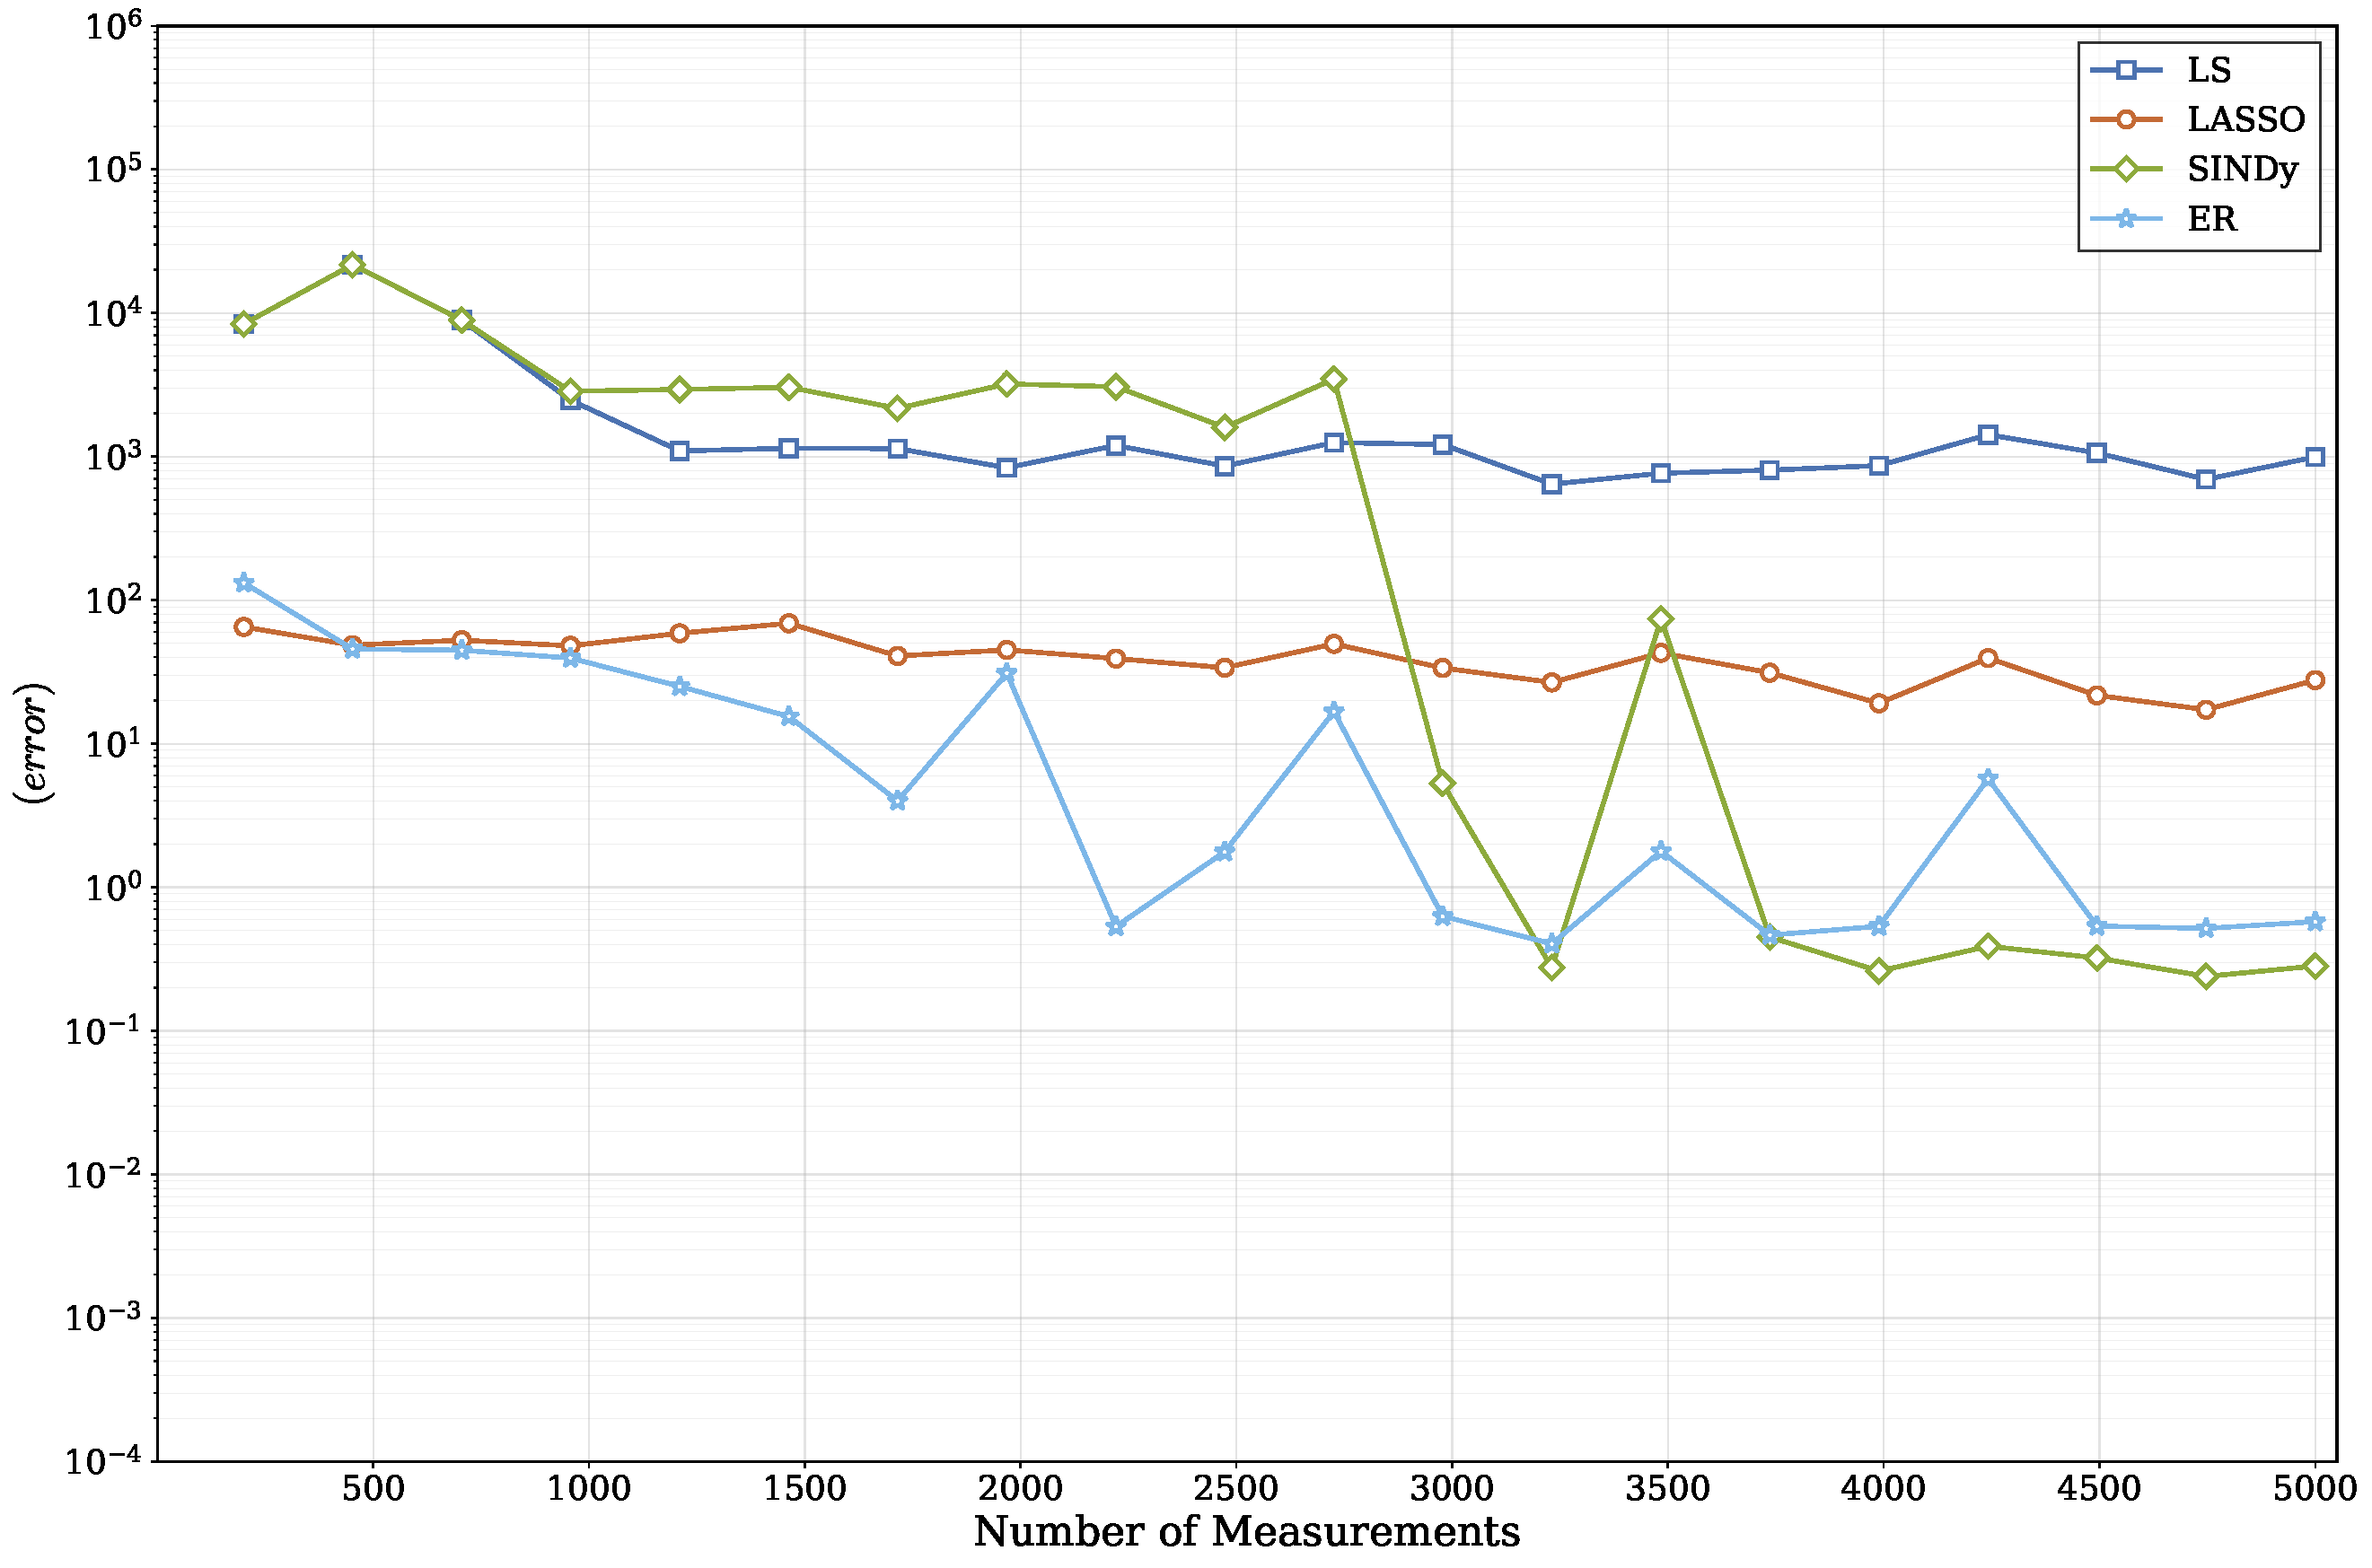
\includegraphics[width=0.7\linewidth]{fig/[FINAL] Fig2.pdf}
    \caption{Figure 2. Comparison of parameter-estimation error for the Lorenz system as a function of the number of measurements. The plotted error is the median $||a_{true} - a_{est}||_2$ over $10$ independent runs, using a time step of $0.0005$, Gaussian measurement noise $\epsilon = 10^{-4}$, no outliers, and a 5th-order polynomial library. Results are shown for LS, LASSO, SINDy, and ER, with error displayed on a logarithmic scale. SINDy requires approximately $3000$ observations to reach the error level achieved by ER, while LASSO remains relatively consistent across sample sizes but never attains ER performance. LS also remains consistent but at significantly higher error levels.}
    \label{fig:fig2}
\end{figure}

To validate the correctness and fidelity of the proposed ERpy implementation, we reproduce the benchmark experiment on the Lorenz system presented in \cite{almomani2020entropic}. The primary objective of this experiment is not to establish new performance claims, but rather to verify that the Python implementation yields results consistent with the original MATLAB-based framework.

We follow the experimental protocol described in the original paper as closely as possible. Specifically, we consider the Lorenz system with standard parameters $\sigma = 10$, $\rho = 28$, and $\beta = 8/3$, and construct a candidate library using a 5th-order polynomial expansion. Time series data are generated using a time step of $0.0005$, and Gaussian measurement noise with variance $\epsilon = 10^{-4}$ is added to the observed states. Derivatives are estimated via finite differences, and parameter estimation error is evaluated using the $\ell_2$ norm between true and estimated coefficients. Results are aggregated over multiple independent runs using the median, consistent with the original study. Unlike the original paper that runs 100 independent simulations, in this work we decided to use 10 independent runs to achieve faster results.

Figure \ref{fig:fig2} shows the parameter estimation error as a function of the number of measurements for LS, LASSO, SINDy, and ER. Qualitatively, the trends observed in our implementation closely match those reported in the original work (see Fig.~2 in \cite{almomani2020entropic}). In particular, ER exhibits significantly improved sample efficiency, achieving low estimation error with substantially fewer measurements compared to competing methods. As in the original study, SINDy requires a considerably larger number of observations (on the order of several thousand) to reach error levels comparable to ER, while LASSO and LS remain relatively stable but at higher error levels.

Moreover, the relative ordering of methods is preserved. These observations are consistent with the conclusions of \cite{almomani2020entropic}, where ER is shown to achieve accurate reconstruction with significantly fewer samples under noisy conditions.

While minor quantitative discrepancies are expected due to differences in implementation details (such as numerical solvers, randomness in data generation, and parameter tuning) the overall agreement in both trend and magnitude of the error curves confirms that \texttt{ERpy} faithfully reproduces the behavior of the original Entropic Regression algorithm.

This result provides strong evidence that the proposed Python implementation correctly captures the core components of ER, including the forward-backward selection procedure and the residual-based evaluation of mutual information, thereby enabling reproducible and extensible experimentation within the Python ecosystem.

\subsection{Mutual Information Estimators}

\begin{figure}[tbp]
    \centering
    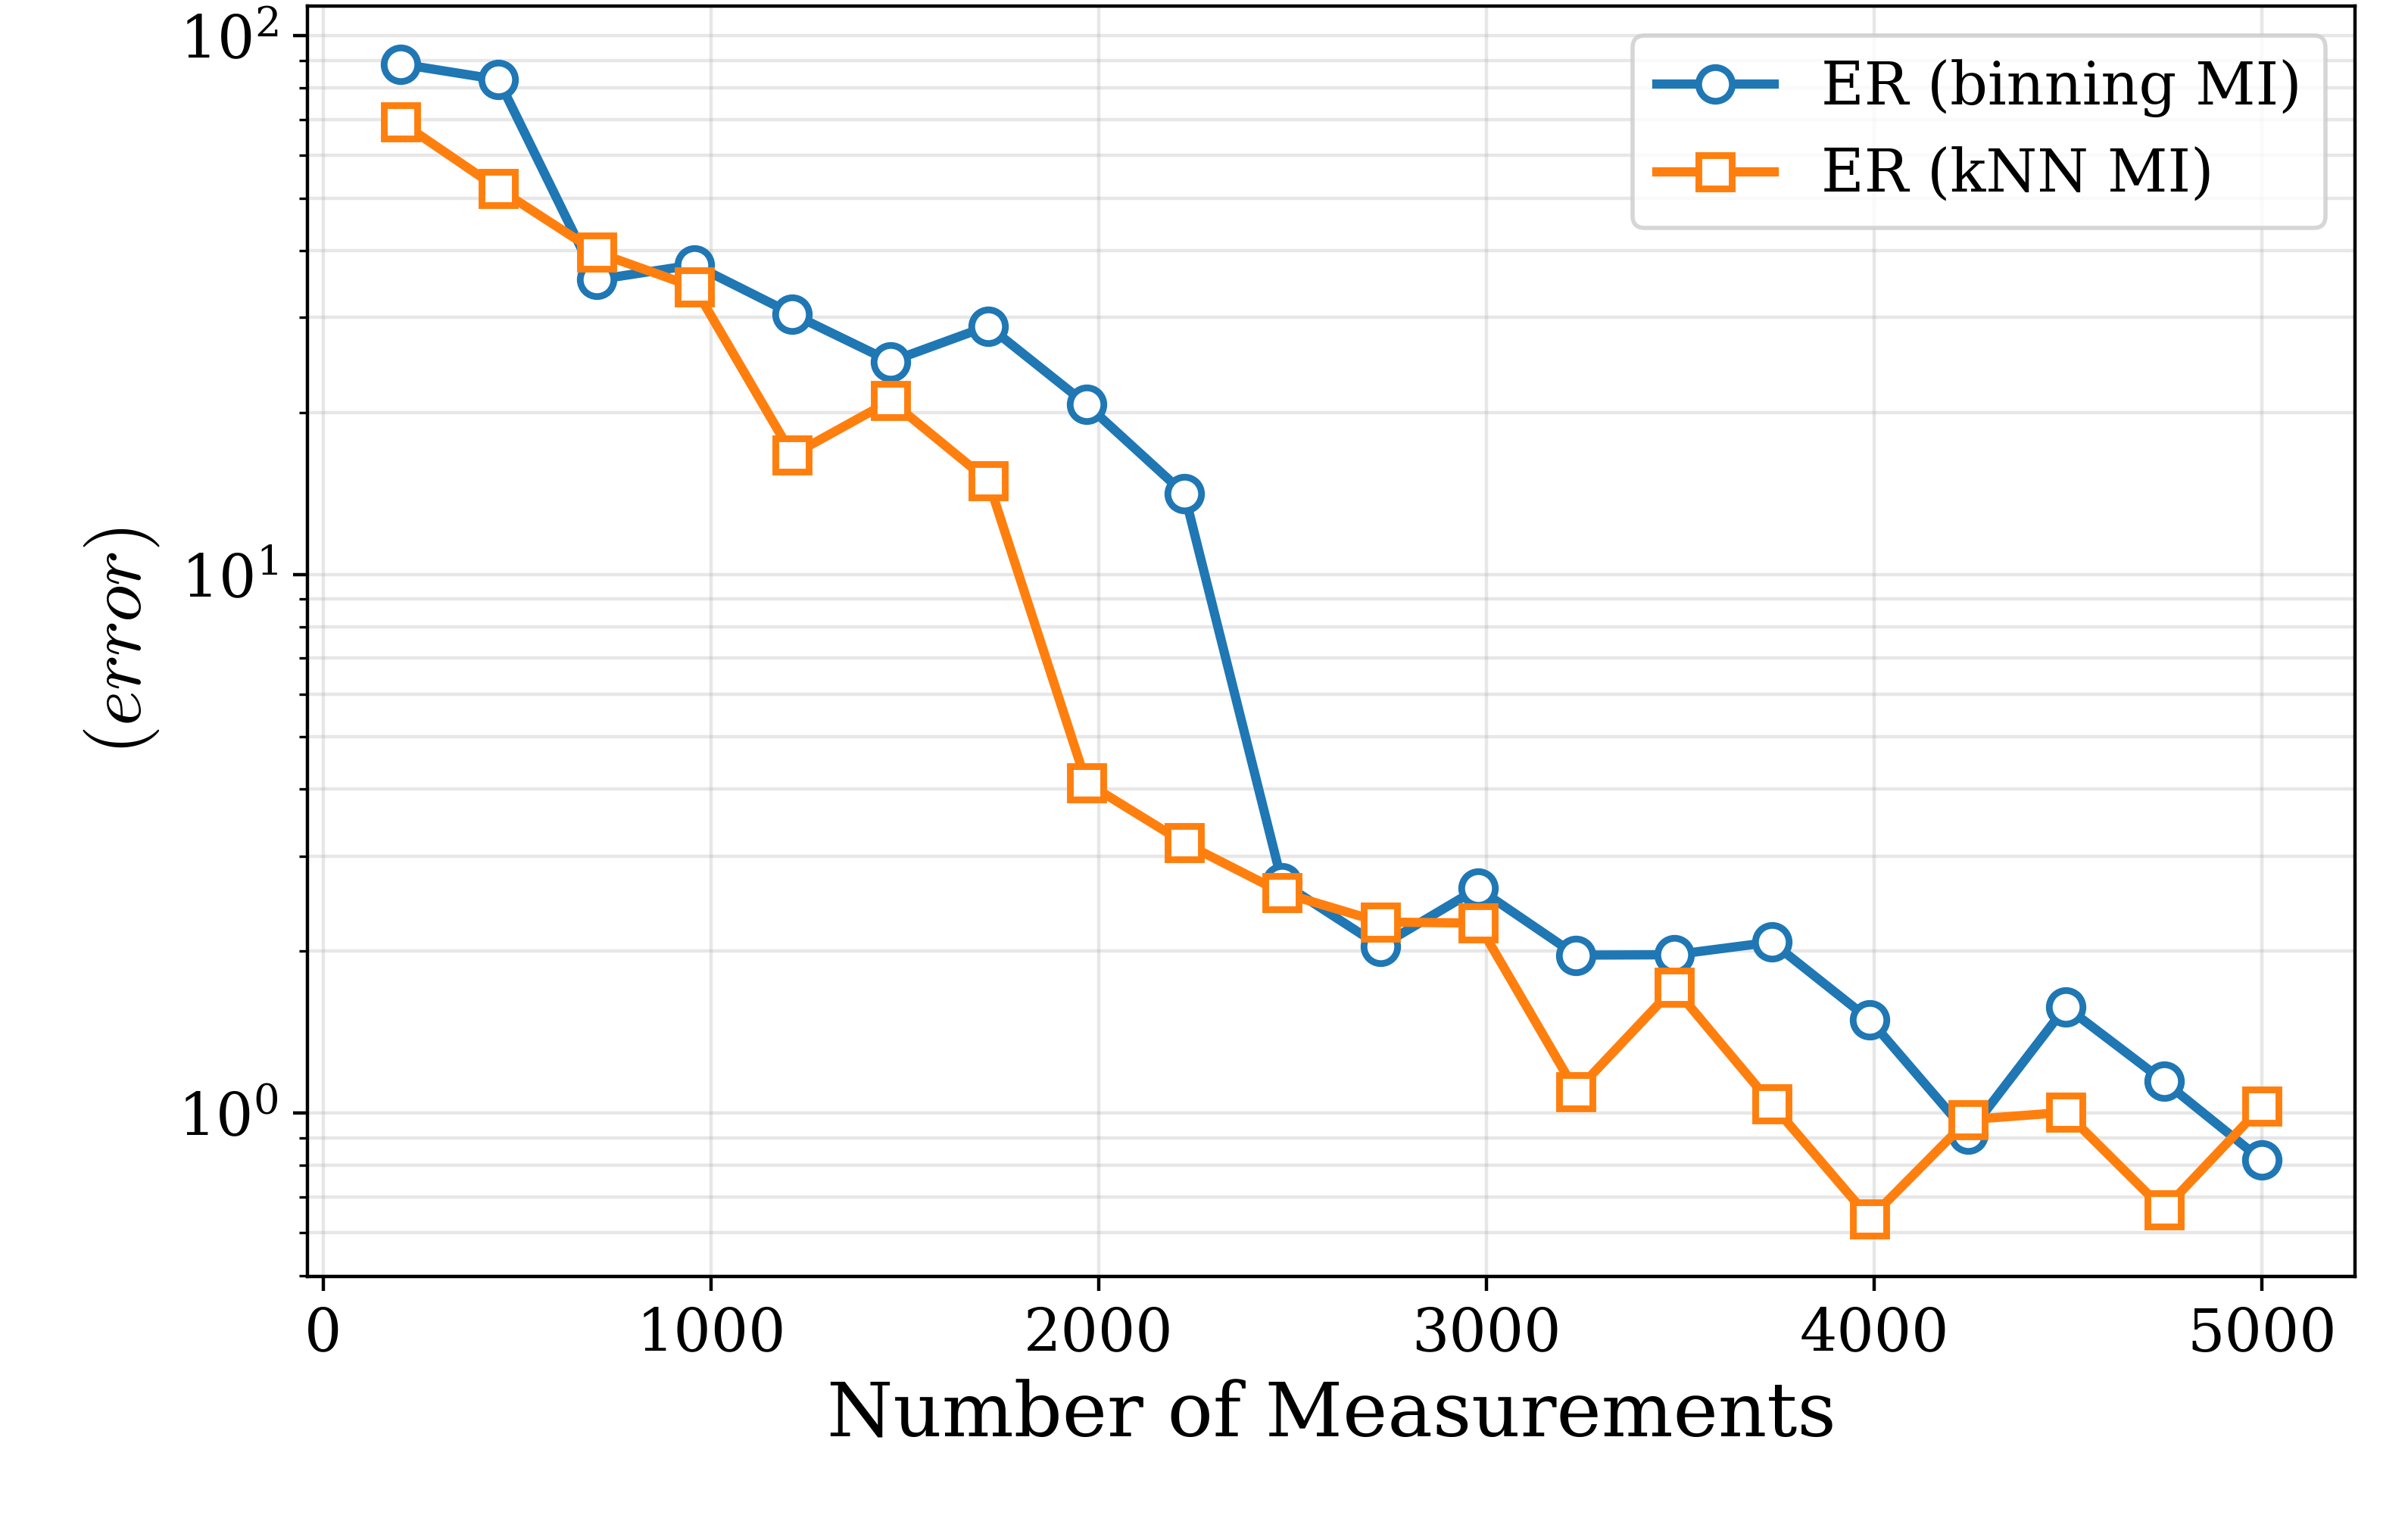
\includegraphics[width=0.7\linewidth]{fig/compare_binning_vs_knn.png}
    \caption{Comparison of Entropic Regression (ER) performance using two binning-based (discrete histogram) and k-nearest neighbor (kNN) mutual information (MI) estimators on the Lorenz system as a function of the number of measurements. The reported error is the median $\ell_2$ norm of the coefficient estimation error, computed over 100 independent runs. The experimental protocol consists of independent simulations with measurement sizes ranging from 200 to 5000 samples, using a time step of 0.0005, Gaussian measurement noise with variance $\epsilon = 10^{-4}$, and a 5th-order polynomial library for system identification. For each measurement size, multiple runs are performed with different random seeds, and results are aggregated via the median to ensure robustness. Overall, the kNN MI estimator consistently achieves lower error than the binning-based estimator and reaches low-error regimes with significantly fewer measurements, highlighting its superior sample efficiency and estimation accuracy in ER.}
    \label{fig:mi_estimators}
\end{figure}

A key component of the Entropic Regression (ER) framework is the estimation of mutual information (MI) and conditional mutual information (CMI) from finite data. In this work, we extend the original framework by systematically comparing two classes of nonparametric MI estimators: (i) discrete binning-based estimators and (ii) k-nearest neighbor (kNN) estimators.

The binning-based approach estimates entropy and mutual information by discretizing continuous variables into a finite number of bins and computing empirical probability mass functions. While simple and computationally efficient, this method is known to suffer from bias due to discretization and sensitivity to the choice of bin size, particularly in high-dimensional or small-sample regimes.

In contrast, the kNN-based estimator estimates MI directly from inter-sample distances without explicit discretization. This method adapts naturally to the local geometry of the data distribution and has been shown to provide more accurate and sample-efficient estimates of information-theoretic quantities, especially for continuous variables.

To assess the impact of the MI estimator on ER performance, we conduct a controlled comparison using the Lorenz system benchmark under identical experimental conditions. As shown in Figure \ref{fig:mi_estimators}, the choice of estimator has an effect on the accuracy and convergence behavior of ER. In particular, the kNN-based estimator consistently achieves lower parameter estimation error and reaches low-error regimes with fewer measurements compared to the binning-based approach.

These results highlight that, beyond the ER algorithm itself, the quality of mutual information estimation plays a critical role in model discovery. The modular design of \texttt{ERpy} allows practitioners to easily substitute and evaluate different estimators, providing a flexible platform for further research on information-theoretic system identification.

\section{Conclusion} \label{section4}

In this work, we presented \texttt{ERpy}, a lightweight and faithful Python implementation of the Entropic Regression (ER) framework for nonlinear system identification presented in \cite{almomani2020entropic}. Through numerical experiments on the Lorenz system, we demonstrated that the proposed implementation successfully reproduces the qualitative and quantitative behavior of the original MATLAB-based approach, preserving both the sample efficiency and accuracy advantages of ER over competing methods.

In addition, we highlighted the critical role of mutual information estimation in the overall performance of ER, showing that kNN-based estimators can significantly improve accuracy and convergence compared to traditional binning methods. These findings emphasize not only the robustness of the ER methodology but also the importance of estimator choice in practical applications.

Overall, \texttt{ERpy} provides a reproducible, extensible, and accessible platform for information-theoretic model discovery within the Python ecosystem, enabling future research in sparse system identification and facilitating integration with modern data-driven workflows.

\bibliographystyle{plain}
\bibliography{biblio}

\end{document}
